\documentclass[]{article}
\usepackage[a4paper]{geometry}
\geometry{top=1cm, bottom=1cm, left=1cm, right=1cm}
\usepackage[utf8]{inputenc}
\usepackage{amsmath}
\usepackage{amsfonts}
\usepackage{amssymb}
\usepackage{graphicx}
\usepackage{float}
\usepackage{caption}
\usepackage{subfigure}
\usepackage{multirow} 
%opening
\title{Simulations of the Sitnikov Problem}
\author{}

\begin{document}

\maketitle

%\begin{abstract}

%\end{abstract}
%%$\dot{z}=\dfrac{-z}{\left(z^2+r^2 \left(t;\varepsilon\right)\right)^\frac{3}{2}}$\\
%$r=\frac{1}{2}\left(1-\epsilon cos\left(u\right)\right)$\\
%$t=u-\epsilon sin\left(u\right)$

\section*{Poincaré Maps}

The solution of the differential equation was gotten by apply the Runge-Kutta-Fehtberg Method. For the Poincaré Map the initial conditions are the set of some points over the line $\dot{z_0}=\alpha z$ with $z_0$ between $-1$ to $1$, and $\alpha$ be the slope of the line, in this case $\alpha=1$. The map is composed $1000$ times for each condition. We considered $200$ values of the initial conditions in the interval described above.\\

\noindent For our Poincaré Maps we considered $10$ values of the exccentricity, as follow:
\begin{figure*}[h]
	\centering
	\subfigure[Complete Poincaré Map.]{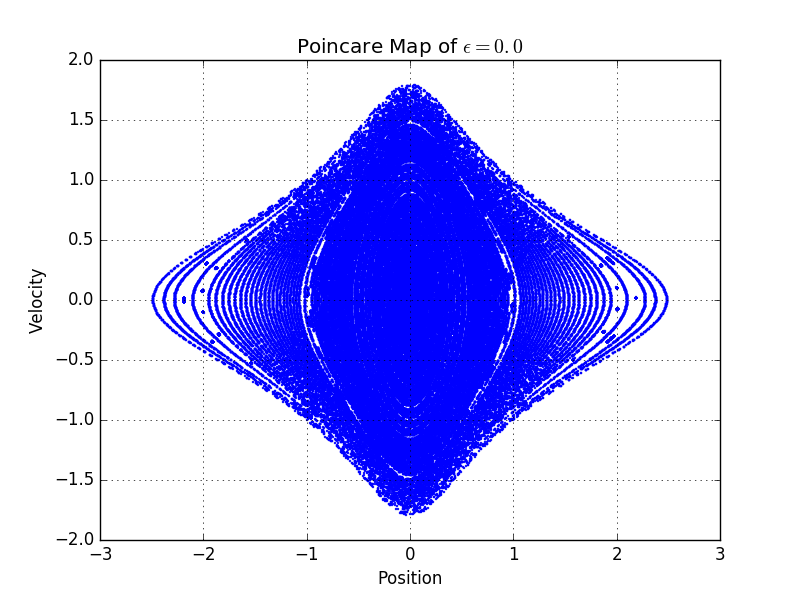
\includegraphics[width=100mm]{/home/alejandra/Dropbox/Mathematics/Investigacion/Master/Queens/Plots/Epsilon(0,0)/MP(0,0)slope(1).png}}
	\caption{Graphics of numerical solution and Poincaré Map with $\epsilon=0.0$..}
\end{figure*}
\begin{figure*}[h]
	\centering
	\subfigure[Complete Poincaré Map.]{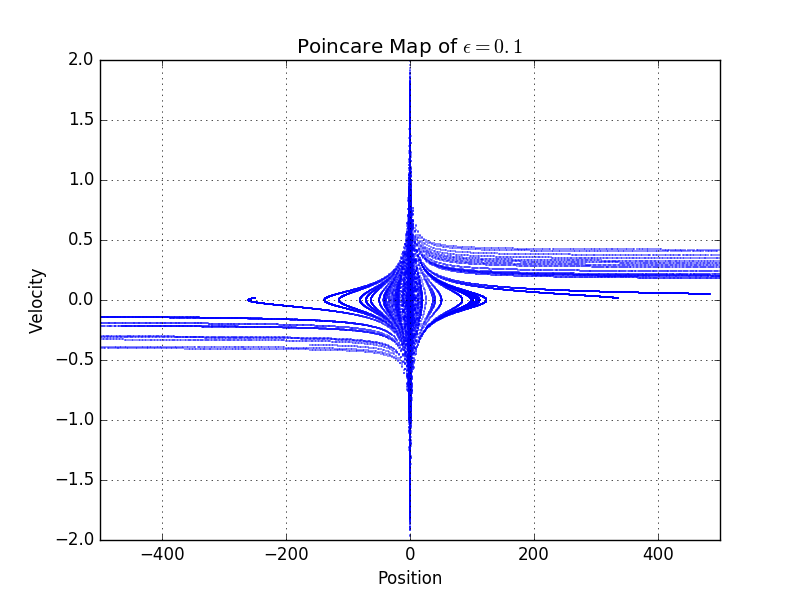
\includegraphics[width=90mm]{/home/alejandra/Dropbox/Mathematics/Investigacion/Master/Queens/Plots/Epsilon(0,1)/MP(0,1)slope(1)3.png}}
	\subfigure[Poincaré Map of position between $-1$ to $1$.]{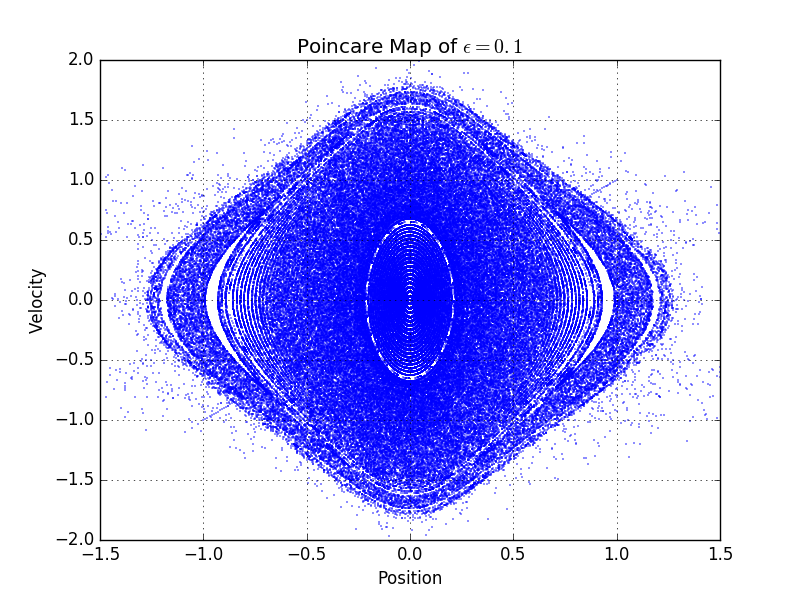
\includegraphics[width=90mm]{/home/alejandra/Dropbox/Mathematics/Investigacion/Master/Queens/Plots/Epsilon(0,1)/MP(0,1)slope(1)2.png}}
	\subfigure[Internal circle of the Poincaré Map.]{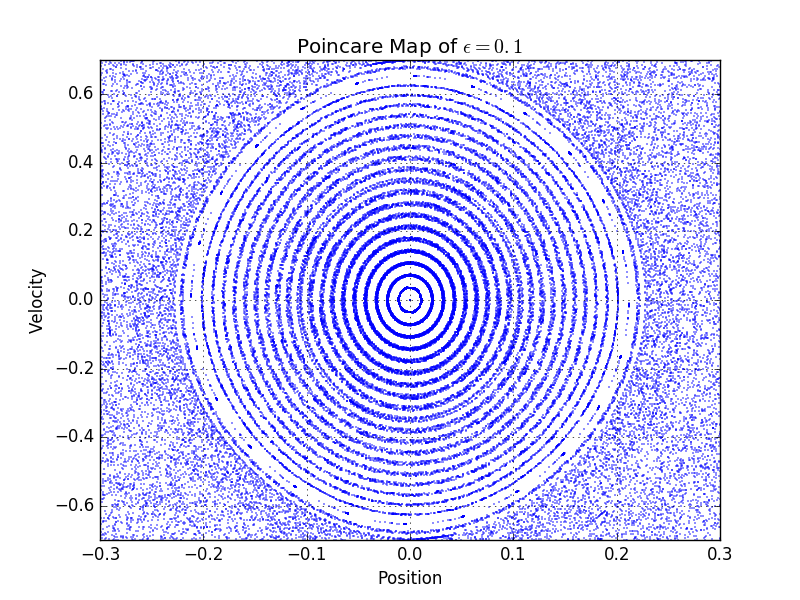
\includegraphics[width=90mm]{/home/alejandra/Dropbox/Mathematics/Investigacion/Master/Queens/Plots/Epsilon(0,1)/MP(0,1)slope(1).png}}
	\caption{Graphics of numerical solution and Poincaré Map with $\epsilon=0.1$.}
\end{figure*}
\begin{figure*}[ht]
	\centering
	\subfigure[Poincaré Map of position between $-1$ to $1$.]{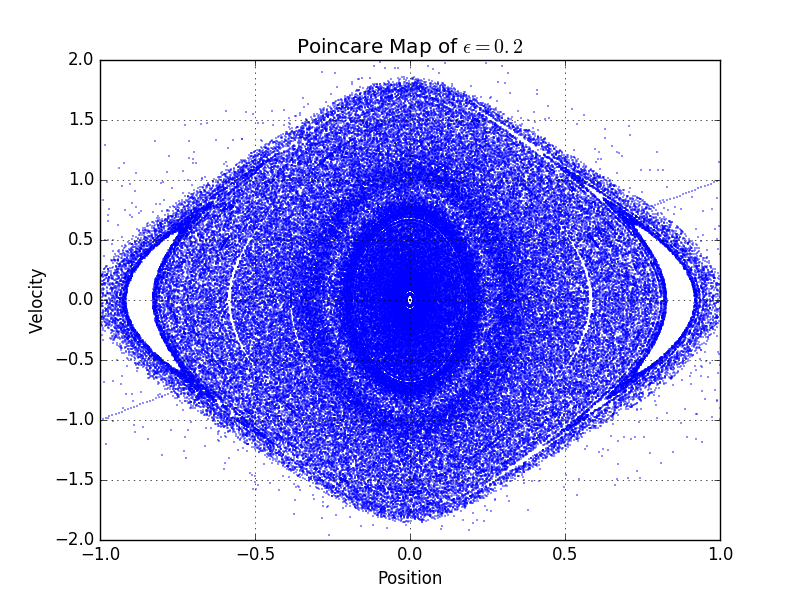
\includegraphics[width=90mm]{/home/alejandra/Dropbox/Mathematics/Investigacion/Master/Queens/Plots/Epsilon(0,2)/MP(0,2)slope(1).png}}
	\subfigure[First Internal circle of the Poincaré Map.]{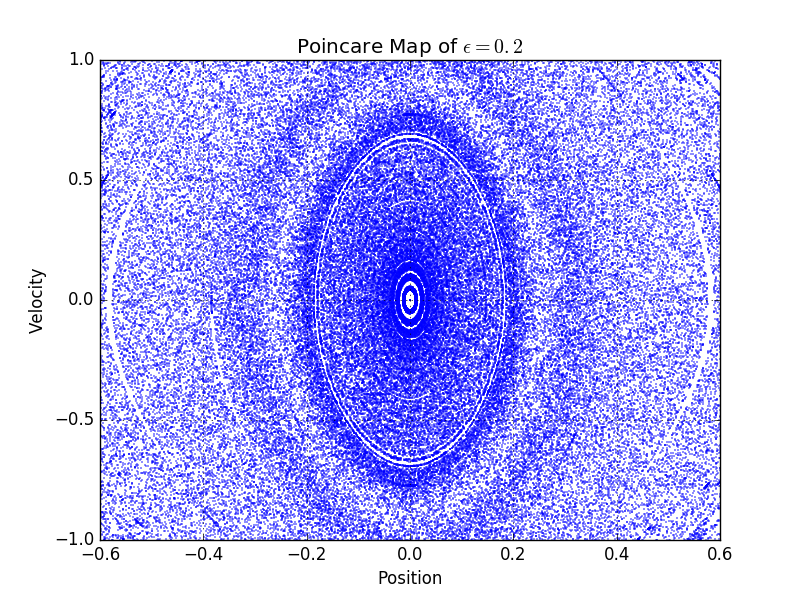
\includegraphics[width=90mm]{/home/alejandra/Dropbox/Mathematics/Investigacion/Master/Queens/Plots/Epsilon(0,2)/MP(0,2)slope(1)2.png}}
	\subfigure[Second Internal circle of the Poincaré Map.]{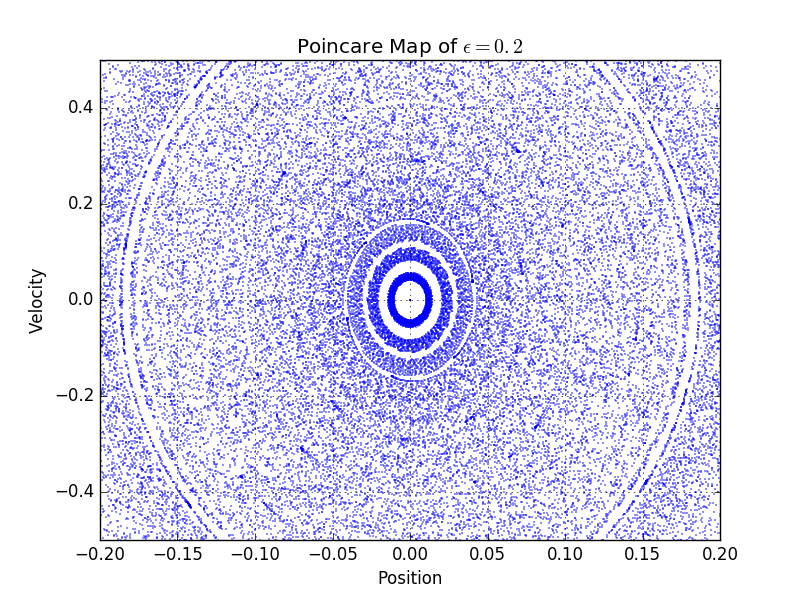
\includegraphics[width=90mm]{/home/alejandra/Dropbox/Mathematics/Investigacion/Master/Queens/Plots/Epsilon(0,2)/MP(0,2)slope(1)3.png}}
	\subfigure[Third Internal circle of the Poincaré Map.]{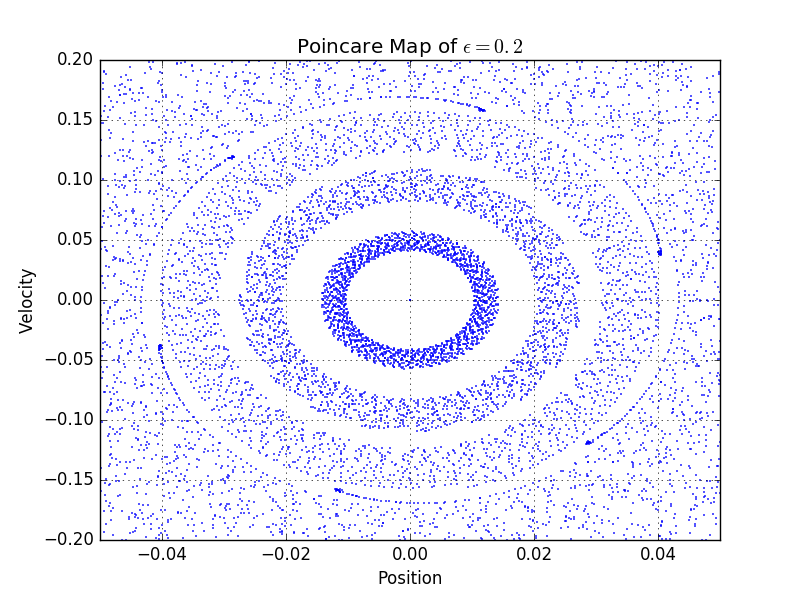
\includegraphics[width=90mm]{/home/alejandra/Dropbox/Mathematics/Investigacion/Master/Queens/Plots/Epsilon(0,2)/MP(0,2)slope(1)4.png}}
	\subfigure[Complete Poincaré Map.]{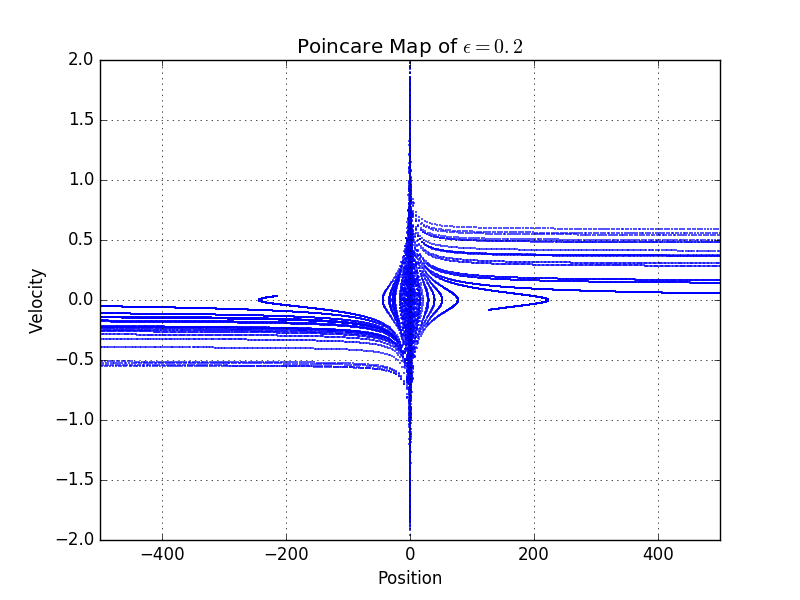
\includegraphics[width=80mm]{/home/alejandra/Dropbox/Mathematics/Investigacion/Master/Queens/Plots/Epsilon(0,2)/MP(0,2)slope(1)5.png}}
	\caption{Graphics of numerical solution and Poincaré Map with $\epsilon=0.2$.}
\end{figure*}
\begin{figure*}[ht]
	\centering
	\subfigure[ Complete Poincaré Map.]{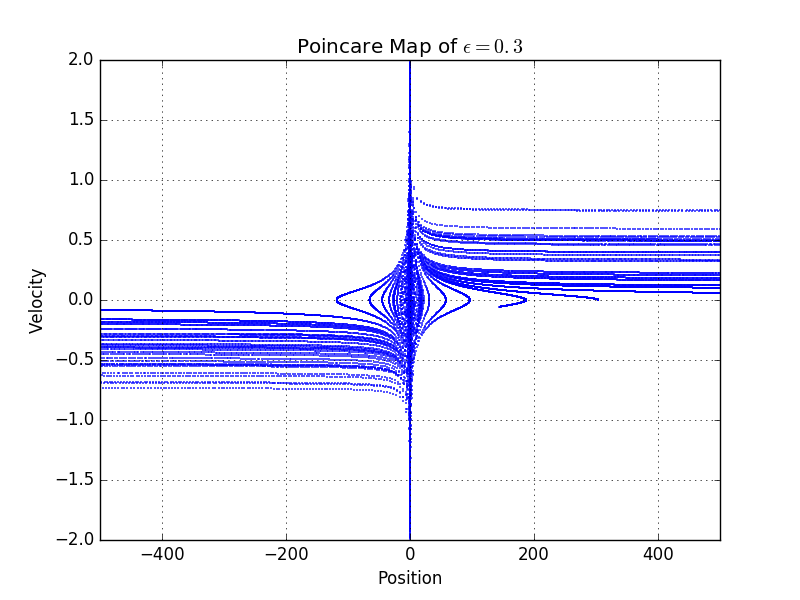
\includegraphics[width=90mm]{/home/alejandra/Dropbox/Mathematics/Investigacion/Master/Queens/Plots/Epsilon(0,3)/MP(0,3)slope(1).png}}
	\subfigure[Poincaré Map of position between $-1$ to $1$.]{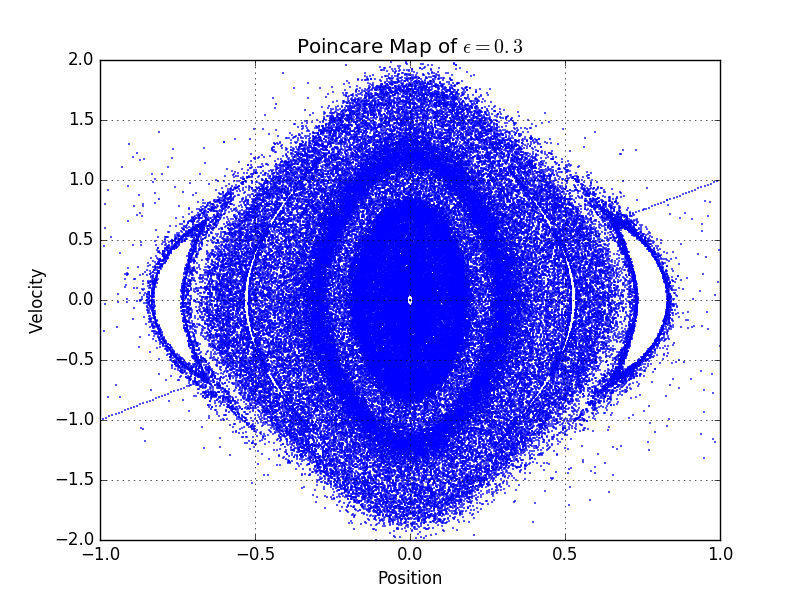
\includegraphics[width=90mm]{/home/alejandra/Dropbox/Mathematics/Investigacion/Master/Queens/Plots/Epsilon(0,3)/MP(0,3)slope(1)2.png}}
	\subfigure[Third Internal circle of the Poincaré Map.]{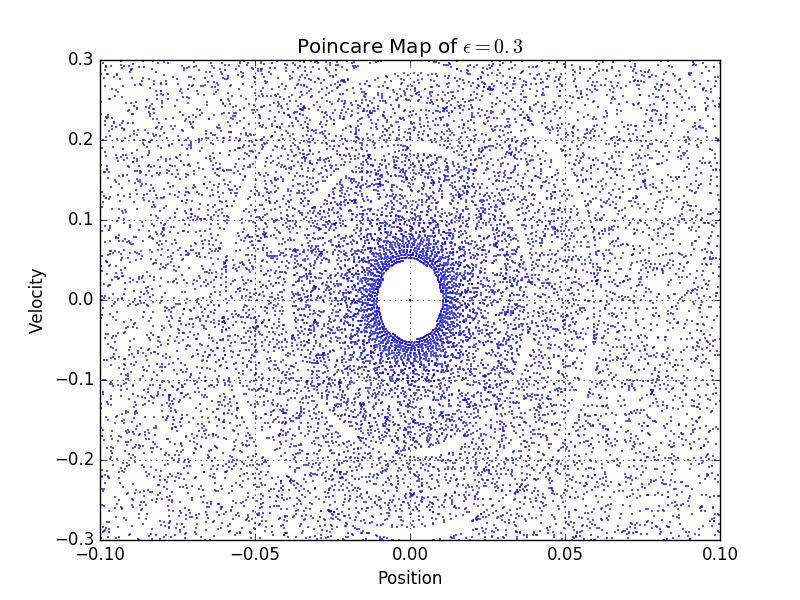
\includegraphics[width=90mm]{/home/alejandra/Dropbox/Mathematics/Investigacion/Master/Queens/Plots/Epsilon(0,3)/MP(0,3)slope(1)4.png}}
	\caption{Graphics of numerical solution and Poincaré Map with $\epsilon=0.3$.}
\end{figure*}
\begin{figure*}[ht]
	\centering
	\subfigure[ Complete Poincaré Map.]{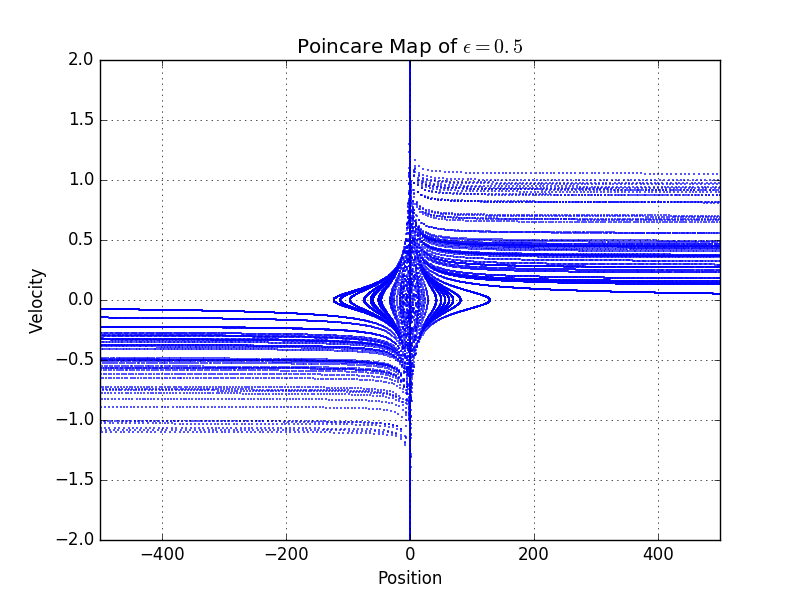
\includegraphics[width=90mm]{/home/alejandra/Dropbox/Mathematics/Investigacion/Master/Queens/Plots/Epsilon(0,5)/MP(0,5)slope(1).png}}
	\subfigure[Poincaré Map of position between $-1$ to $1$.]{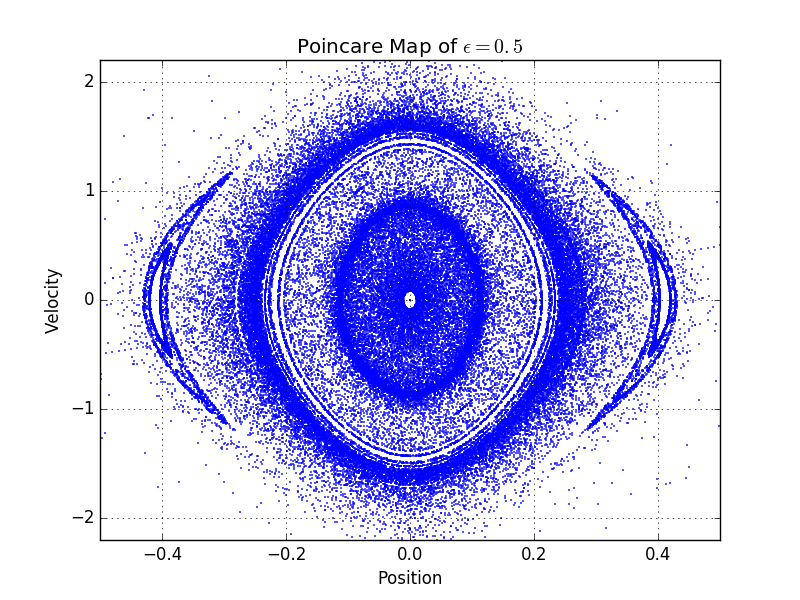
\includegraphics[width=90mm]{/home/alejandra/Dropbox/Mathematics/Investigacion/Master/Queens/Plots/Epsilon(0,5)/MP(0,5)slope(1)2.png}}
	\caption{Graphics of numerical solution and Poincaré Map with $\epsilon=0.5$.}
\end{figure*}
\begin{figure*}[ht]
	\centering
	\subfigure[ Complete Poincaré Map.]{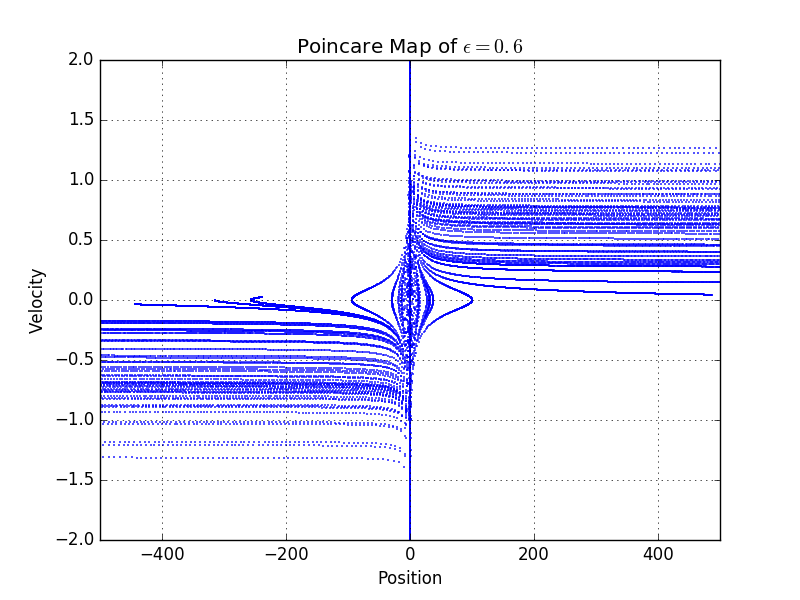
\includegraphics[width=90mm]{/home/alejandra/Dropbox/Mathematics/Investigacion/Master/Queens/Plots/Epsilon(0,6)/MP(0,6)slope(1).png}}
	\subfigure[Poincaré Map of position between $-1$ to $1$.]{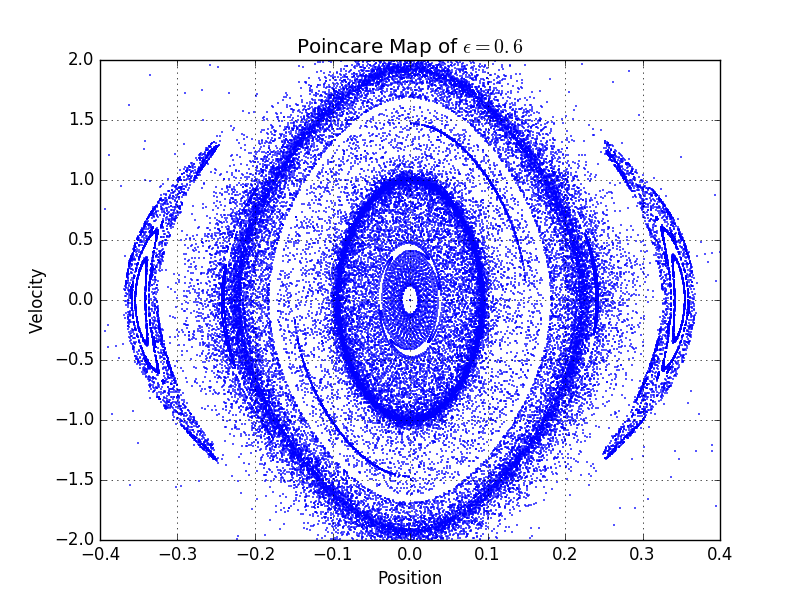
\includegraphics[width=90mm]{/home/alejandra/Dropbox/Mathematics/Investigacion/Master/Queens/Plots/Epsilon(0,6)/MP(0,6)slope(1)2.png}}
	\subfigure[Third Internal circle of the Poincaré Map.]{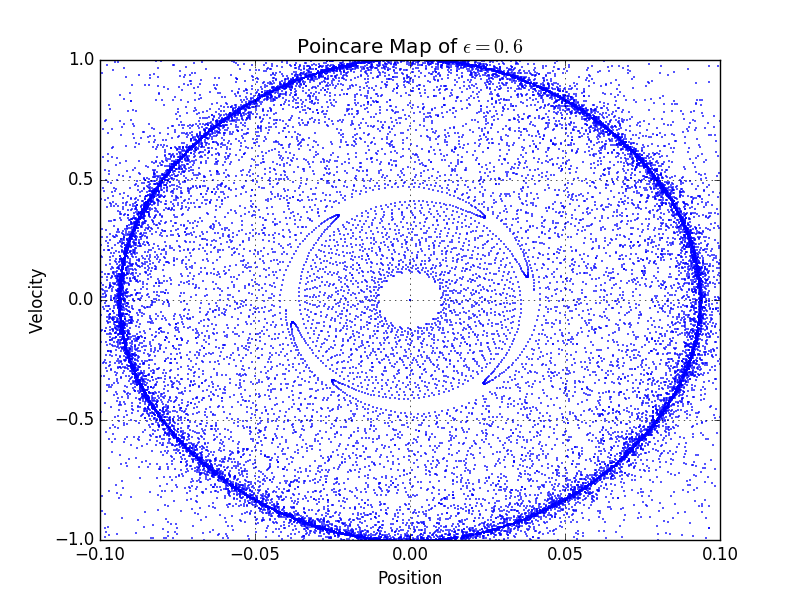
\includegraphics[width=90mm]{/home/alejandra/Dropbox/Mathematics/Investigacion/Master/Queens/Plots/Epsilon(0,6)/MP(0,6)slope(1)4.png}}
	\caption{Graphics of numerical solution and Poincaré Map with $\epsilon=0.6$.}
\end{figure*}
\begin{figure*}[ht]
	\centering
	\subfigure[ Complete Poincaré Map.]{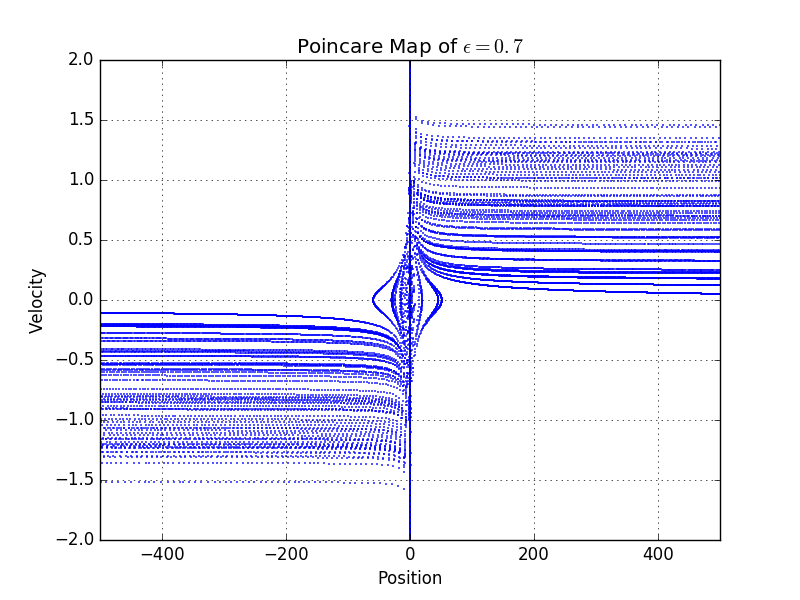
\includegraphics[width=90mm]{/home/alejandra/Dropbox/Mathematics/Investigacion/Master/Queens/Plots/Epsilon(0,7)/MP(0,7)slope(1).png}}
	\subfigure[Complete Poincaré Map near to initial conditions.]{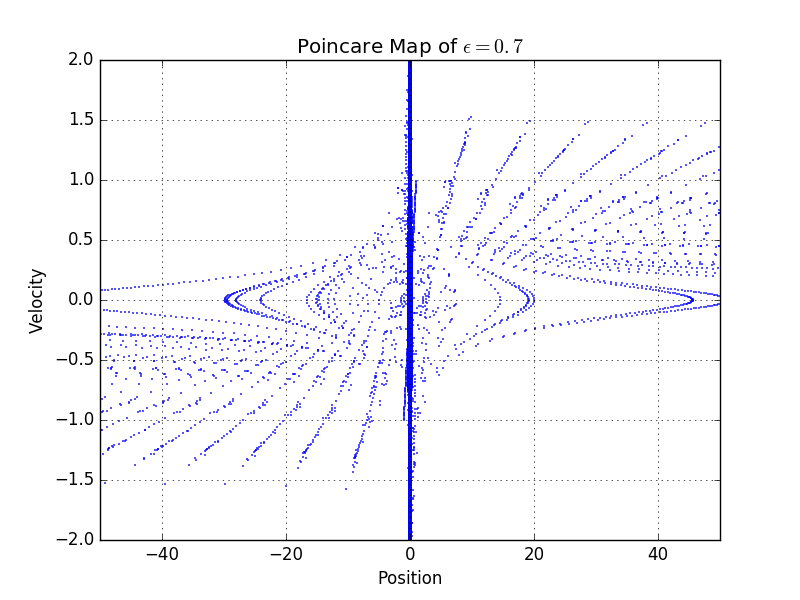
\includegraphics[width=90mm]{/home/alejandra/Dropbox/Mathematics/Investigacion/Master/Queens/Plots/Epsilon(0,7)/MP(0,7)slope(1)2.png}}
	\subfigure[Third Internal circle of the Poincaré Map.]{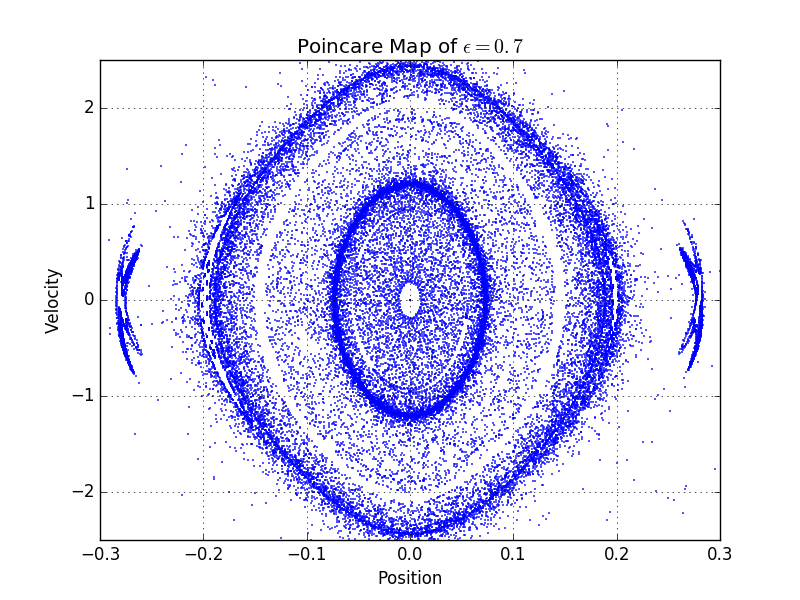
\includegraphics[width=90mm]{/home/alejandra/Dropbox/Mathematics/Investigacion/Master/Queens/Plots/Epsilon(0,7)/MP(0,7)slope(1)3.png}}
	\caption{Graphics of numerical solution and Poincaré Map with $\epsilon=0.7$.}
\end{figure*}

\begin{figure*}[ht]
	\centering
	\subfigure[ Complete Poincaré Map.]{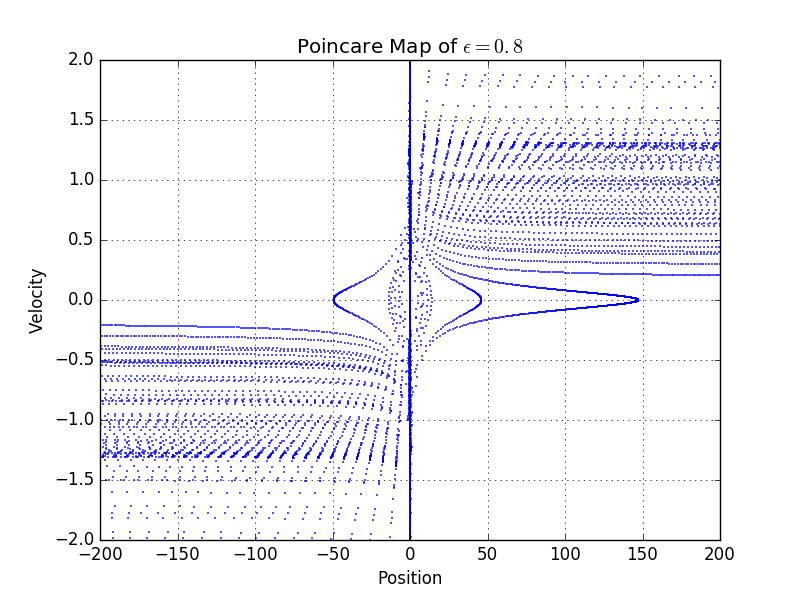
\includegraphics[width=90mm]{/home/alejandra/Dropbox/Mathematics/Investigacion/Master/Queens/Plots/Epsilon(0,8)/MP(0,8)slope(1)2.png}}
	\subfigure[Complete Poincaré Map near to initial conditions.]{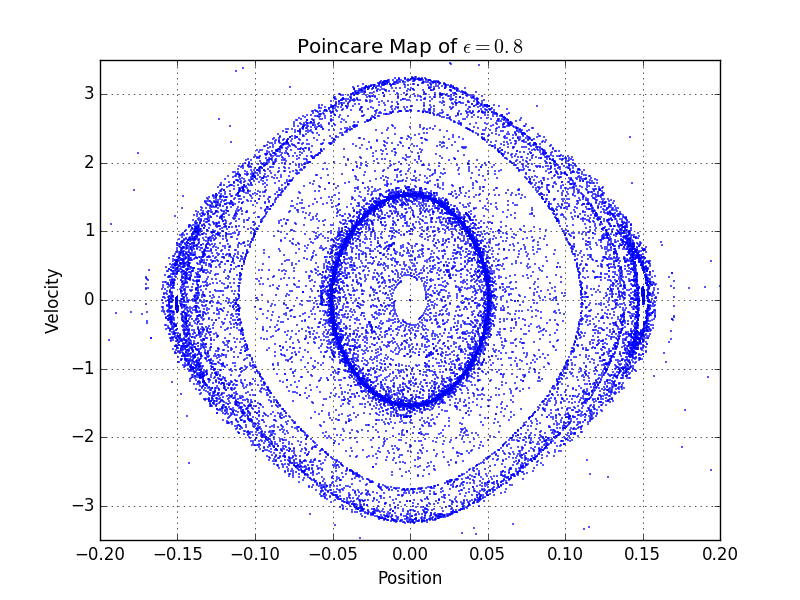
\includegraphics[width=90mm]{/home/alejandra/Dropbox/Mathematics/Investigacion/Master/Queens/Plots/Epsilon(0,8)/MP(0,8)slope(1)3.png}}
	\subfigure[Third Internal circle of the Poincaré Map.]{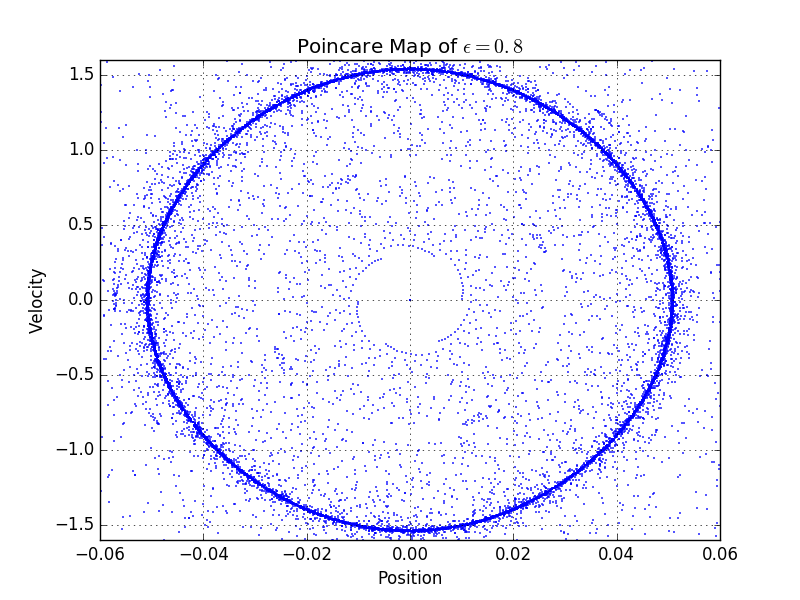
\includegraphics[width=90mm]{/home/alejandra/Dropbox/Mathematics/Investigacion/Master/Queens/Plots/Epsilon(0,8)/MP(0,8)slope(1)4.png}}
	\caption{Graphics of numerical solution and Poincaré Map with $\epsilon=0.8$.}
\end{figure*}
\begin{figure*}[ht]
	\centering
	\subfigure[ Complete Poincaré Map.]{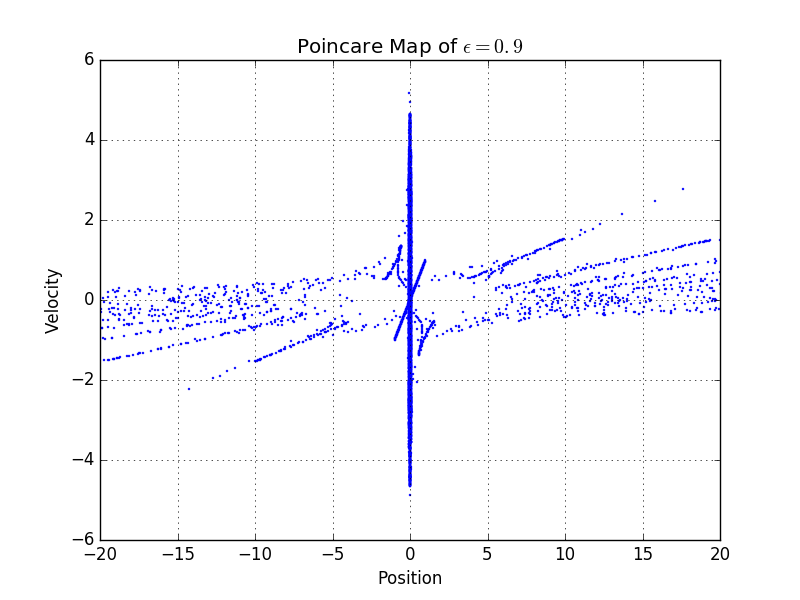
\includegraphics[width=90mm]{/home/alejandra/Dropbox/Mathematics/Investigacion/Master/Queens/Plots/Epsilon(0,9)/MP(0,9)slope(1)2.png}}
	\subfigure[Complete Poincaré Map near to initial conditions.]{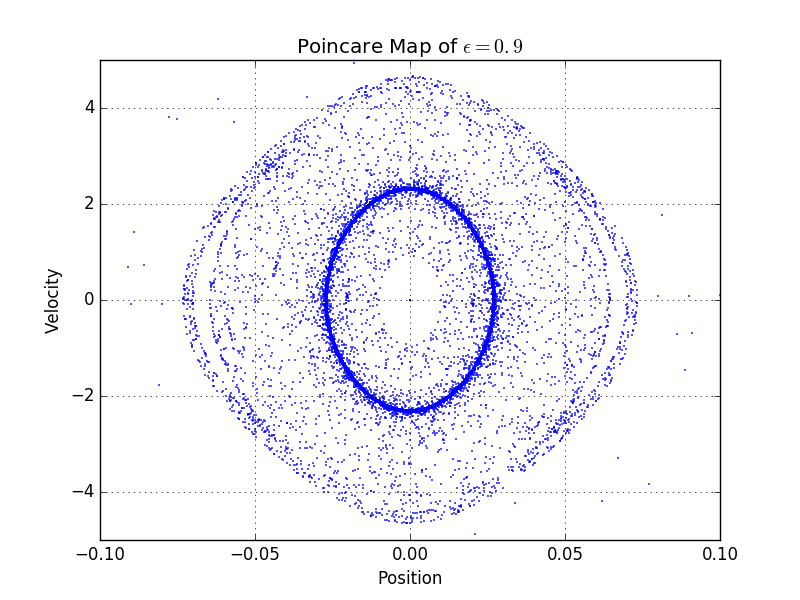
\includegraphics[width=90mm]{/home/alejandra/Dropbox/Mathematics/Investigacion/Master/Queens/Plots/Epsilon(0,9)/MP(0,9)slope(1)3.png}}
	\subfigure[Third Internal circle of the Poincaré Map.]{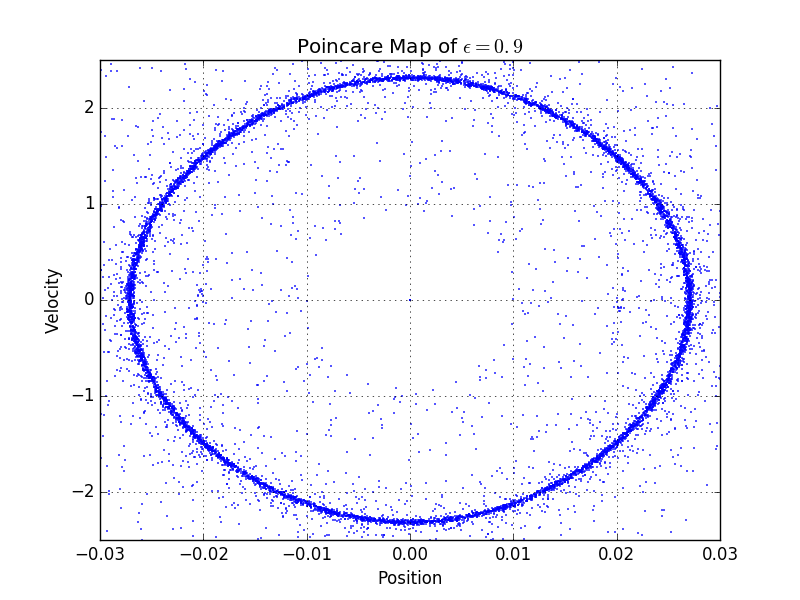
\includegraphics[width=90mm]{/home/alejandra/Dropbox/Mathematics/Investigacion/Master/Queens/Plots/Epsilon(0,9)/MP(0,9)slope(1)4.png}}
	\caption{Graphics of numerical solution and Poincaré Map with $\epsilon=0.9$.}
\end{figure*}
\end{document}
